\documentclass[border=10pt]{standalone}
\usepackage{tikz}
\usetikzlibrary{arrows.meta, shapes, calc}

\begin{document}
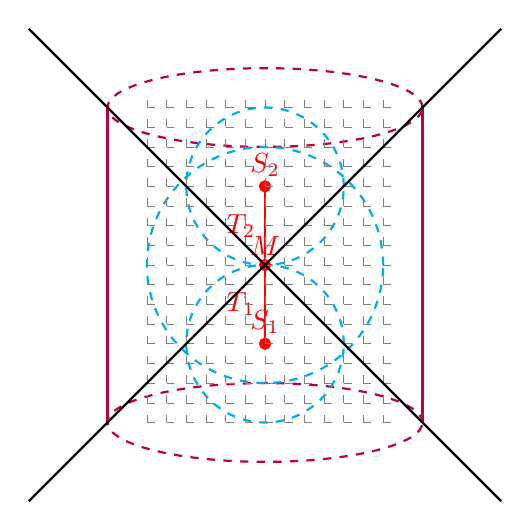
\begin{tikzpicture}
    % Define the main cylinder
    \draw[thick, purple, dashed] (0,0) ellipse (2cm and 0.5cm);
    \draw[thick, purple, dashed] (0,4) ellipse (2cm and 0.5cm);
    \draw[thick, purple] (-2,0) -- (-2,4);
    \draw[thick, purple] (2,0) -- (2,4);

    % Define the spheres
    \draw[thick, cyan, dashed] (0,2) circle (1.5cm);
    \draw[thick, cyan, dashed] (0,1) circle (1cm);
    \draw[thick, cyan, dashed] (0,3) circle (1cm);

    % Define the points and lines
    \filldraw[red] (0,2) circle (2pt) node[above] {$M$};
    \filldraw[red] (0,1) circle (2pt) node[above] {$S_1$};
    \filldraw[red] (0,3) circle (2pt) node[above] {$S_2$};
    \draw[red] (0,2) -- (0,1) node[midway, left] {$T_1$};
    \draw[red] (0,2) -- (0,3) node[midway, left] {$T_2$};

    % Define the grid
    \foreach \x in {-1.5,-1.25,...,1.5}
    \foreach \y in {0,0.25,...,4}
    {
        \draw[gray, very thin] (\x,\y) -- (\x+0.1,\y);
    }
    \foreach \y in {0,0.25,...,4}
    \foreach \x in {-1.5,-1.25,...,1.5}
    {
        \draw[gray, very thin] (\x,\y) -- (\x,\y+0.1);
    }

    % Define the perspective lines
    \draw[thick] (-3,-1) -- (3,5);
    \draw[thick] (-3,5) -- (3,-1);

\end{tikzpicture}
\end{document}